\documentclass[eikonal.tex]{subfiles}

\begin{document}

\section{Constrained Newton's Method for Minimizing $F_0$ and
  $F_1$}\label{sec:constrained-newton}

Except for $F_0$ in special cases, $F_0$ and $F_1$ are nonlinear and
nonquadratic functions. The function $F_0$ is convex, but the same
can't be said for $F_1$. We explored a variety of methods for
minimizing these functions, and the sequential quadratic programming
(SQP) framework ended up being one of the most reliable. The
minimization problem to solve is:
\begin{align*}
  \mbox{minimize} & \qquad F_i(\lambda; \theta) \\
  \mbox{subject to} & \qquad \lambda \in \Delta^d
\end{align*}
for $i = 0, 1$. Let $k$ be the iteration number and let $\lambda_k$ be
the $k$th iterate. If we expand $F_i$:
\begin{align}\label{eq:Fi-taylor-expansion}
  F_i(\lambda; \theta) = F_i(\lambda_k; \theta) + \nabla_\lambda F_i(\lambda_k; \theta)^\top (\lambda - \lambda_k) + \frac{1}{2} {(\lambda - \lambda_k)}^\top \nabla_\lambda^2 F_i(\lambda_k; \theta) {(\lambda - \lambda_k)} + O(\norm{\lambda - \lambda_k}^3),
\end{align}
then formulating our problem as an SQP requires that we form a
sequence of iterates by approximating $F_i$ using the first three
terms of \cref{eq:Fi-taylor-expansion} and solving the
inequality-constrained quadratic program (QP):
\begin{align*}
  \mbox{minimize} & \qquad F_i(\lambda_k; \theta) + \nabla_\lambda F_i(\lambda_k; \theta)^\top (\lambda - \lambda_k) + \frac{1}{2} {(\lambda - \lambda_k)}^\top \nabla_\lambda^2 F_i(\lambda_k; \theta) {(\lambda - \lambda_k)} \\
  \mbox{subject to} & \qquad \lambda \in \Delta^d.
\end{align*}
The solution of this problem can be carried out in a variety of
ways. Since we are interested in small values of $d$ (in particular,
$d = 2$), and since the number of constraints is $d + 1 = O(d)$, a
suitable approach is to use the active set method. At each step of the
active set method, an equality-constrained QP is solved. For $F_0$,
this is straightforward, and can again be accomplished in a variety of
ways; for $F_1$, the Hessian $\nabla_\lambda^2 F_1$ can be indefinite,
which requires us to perturb it to ensure descent.

\paragraph{An informal description of the algorithm.} In this section,
we sketch the update algorithm in broad strokes. Since $\Delta^d$ is a
polytope, we can write $\lambda \in \Delta^d$ as a linear matrix
inequality:
\begin{align*}
  A\lambda \leq b, \mbox{ where } A = \begin{pmatrix}
    -I \\ \m{1}_{1 \times d}
  \end{pmatrix} \mbox{ and } b = \begin{pmatrix}
    \m{0}_{d \times 1} \\ 1
  \end{pmatrix}.
\end{align*}
The main procedures comprising the update algorithm follow.
\begin{enumerate}
\item \textbf{SQP iteration.} We start by computing
  $G_k = \nabla^2 F_i(\lambda_k)$. If $G_k$ is indefinite, we perturb
  $G_k \gets G_k + \epsilon I$ so that
  $\lambda_{\operatorname{min}}(G_k + \epsilon I) > 0$. Next, we
  compute the gradient $g_k = \nabla_\lambda F_i(\lambda_k)$ and the
  load vector for the iteration, $c_k = g_k - G_k \lambda_k$. If
  we write $F_k = F_i(\lambda_k)$, then our quadratic approximation to
  our cost function can be written
  $\tfrac{1}{2} \lambda^\top G_k \lambda + c_k^\top \lambda + C_k$,
  where $C_k$ is a constant. Solving the problem:
  \begin{equation}\label{eq:iqp}
    \begin{aligned}
      \mbox{minimize} & \qquad \frac{1}{2} \lambda^\top G_k \lambda + c_k^\top \lambda \\
      \mbox{subject to} & \qquad A\lambda \leq b,
    \end{aligned}
  \end{equation}
  we obtain $\lambda^*$, and write
  $\lambda_{k+1} = \lambda_k + \alpha_k (\lambda^* - \lambda_k)$. The
  quantity $p_k = \lambda^* - \lambda_k$ is the descent direction for
  the step, and $\alpha_k$ is the step length. We note that our method
  of solving \cref{eq:iqp} recovers $-p_k$ instead of $\lambda*$. To
  ensure descent, we use a backtracking procedure to select
  $\alpha_k$, starting with $\alpha_k = 1$.
\item \textbf{Active set iteration.} We solve \cref{eq:iqp} using the
  active set method, which is similar to the simplex algorithm. Our
  method follows the procedures outlined in Chapter 16 of Nocedal and
  Wright~\cite{nocedal2006numerical} and Chapter 2 of
  Bertsekas~\cite{bertsekas1999nonlinear}. The key detail here is
  that, at each iteration of the active set method, an
  equality-constrained QP is solved. The indices of the constraints
  (i.e., the rows of $A \lambda \leq b$) are $\set{1, \hdots, d +
    1}$. A constraint is active for an iterate if it holds with
  equality. Let $I \subseteq \set{1, \hdots, d + 1}$ be the index of
  active constraints for a given iterate, and let $A_I$ denote the
  submatrix consisting of the rows of $A$ indexed by $I$; define $b_I$
  likewise. Then, the equality-constrained QP is:
  \begin{equation}
    \label{eq:eqp}
    \begin{aligned}
      \mbox{minimize} & \qquad \frac{1}{2} \lambda^\top G_k \lambda + c_k^\top \lambda \\
      \mbox{subject to} & \qquad A_I \lambda = b_I.
    \end{aligned}
  \end{equation}
  There are several direct methods for solving equality-constrained
  QPs. Their relative merits depend on the problem being solved. We
  discuss our choice next.
\item \textbf{Solving the equality-constrained quadratic subproblem.}
  If a basis for the so-called nullspace of $A_I$ is easily obtained,
  then one method that is of practical use is the nullspace method,
  described in section 16.2 of Nocedal and
  Wright~\cite{nocedal2006numerical}. A brief description follows. The
  problem given by \cref{eq:eqp} is equivalent to the system:
  \begin{equation}
    \label{eq:kkt-eqp}
    \begin{aligned}
      \begin{pmatrix}
        G_k & A_I^\top \\
        A_I &
      \end{pmatrix} \begin{pmatrix}
        -p_k \\ \gamma^*
      \end{pmatrix} = \begin{pmatrix}
        g_k \\ h_I
      \end{pmatrix},
    \end{aligned}
  \end{equation}
  where $\lambda^*, \gamma^*$ are the solution and Lagrange
  multipliers for \cref{eq:eqp}, $p_k = \lambda^* - \lambda_k$, $g_k$
  is as given above, and $h_I = A_I \lambda_k - b_k$. If we let $Z$ be
  a nullspace matrix for $A_I$ (i.e. such that $A_IZ = 0$), and let
  $Y$ be a matrix such that $\begin{pmatrix} Y & Z \end{pmatrix}$ is
  full rank, blocking $p_k$ so that:
  \begin{align*}
    p_k = \begin{pmatrix} Y & Z \end{pmatrix} \begin{pmatrix}
      p_Y \\ p_Z
    \end{pmatrix} = Y p_Y + Z p_Z
  \end{align*}
  and substituting this into \cref{eq:kkt-eqp} yields the system:
  \begin{align*}
    A_I Y p_Y &= -h_I, \\
    Z^\top G_k Z p_Z &= -Z^\top G_k Y p_Y - Z^\top g_k.
  \end{align*}
  The key to the efficiency of this method in our case is that the
  simplicity of $A$ leads to simple expressions for $Z$ and $Y$, which
  allows these two systems to be solved rapidly.
\end{enumerate}

In the following lemma we show that $Y$ and $Z$ can take very simple
forms (although these forms are not unique). Using these forms,
multiplication by $Y$, $Z$, and $Z^\top$ amount to indexing
operations, and---if $d + 1 \in I$---taking simple differences of
elements. \textbf{TODO}: \emph{MATLAB experiments tell me that
  indexing written in matrix form is compatible with solving a system
  using a Cholesky factorization or a QR decomposition. This is
  extremely useful! I don't think I've checked if it also works for
  the case when $d + 1 \in I$, but I think something straightforward
  should be possible.}

\begin{lemma}\label{lemma:Z}
  Let $I \subseteq \set{1, \hdots, d + 1}$, let $m = |I|$, and let $A$
  be the constraint matrix for $\Delta^d$. Then a nullspace matrix
  $Z \in \set{0, -1, 1}^{d \times d - m}$ for $A$ is given explicitly
  by the following two cases. In both cases, let
  $j_1 < \cdots < j_{d - m}$ be the sorted elements of
  $\set{1, \hdots, d} \backslash I$:
  \begin{enumerate}
  \item If $I \subseteq \set{1, \hdots, d}$, then
    $Z = \begin{pmatrix} e_{j_1} & \cdots &
      e_{j_{d-m}} \end{pmatrix}$.
  \item If $d + 1 \in I$, then
    $Z = \begin{pmatrix} e_{j_2} - e_{j_1} & \cdots & e_{j_{d-m}} -
      e_{j_1}
      \end{pmatrix}$.
  \end{enumerate}
\end{lemma}

\begin{proof}
  \textbf{TODO}: easy.
\end{proof}

\begin{corollary}
  For each $Z$ in \cref{lemma:Z}, a matrix $Y$ such that
  $\begin{pmatrix} Y & Z \end{pmatrix}$ is full rank can be written
  such that its columns are distinct columns of the identity
  matrix. In particular, for each case of \cref{lemma:Z}:
  \begin{enumerate}
  \item If $I \subseteq \set{1, \hdots, d}$, let $i_1 < \cdots < i_m$
    be the sorted elements of $I$. Then, choose
    $Y = \begin{pmatrix} e_{i_1} & \cdots & e_{i_m} \end{pmatrix}$.
  \item If $d + 1 \in I$, let $i_1 < \cdots < i_{m-1}$ be the sorted
    elements of $I \backslash \set{d + 1}$. Then,
    $Y = \begin{pmatrix} e_1 & e_{i_1} & \cdots &
        e_{i_{m-1}} \end{pmatrix}$ suffices.
  \end{enumerate}
\end{corollary}

% \section{An Efficient Update Algorithm for Higher Dimensions}

% \emph{For now, this section is just an outline of a method for solving
%   this problem in higher dimensions that I would like to try
%   implementing.}

% The barycentric simplex constraints are:
% \begin{align*}
%   \m{A} \m{\lambda} \leq \m{b}, \qquad \mbox{where} \qquad \m{A} = \begin{pmatrix}
%     \m{I}_d \\ -\m{1}_{1 \times d}
%   \end{pmatrix}, \qquad \mbox{and} \qquad \m{b} = \begin{pmatrix}
%     \m{0}_{d \times 1} \\ -1
%   \end{pmatrix}.
% \end{align*}
% While solving the a quadratic program with inequality constraints
% specified by $\m{A} \m{\lambda} \leq \m{b}$ using the active set
% method, we have a set of active indices,
% $I \subseteq [1, \hdots, d + 1]$, available to us at each step of the
% iteration. Denote the current set of active constraints by $\m{A}_I$
% and $\m{b}_I$.  To use the ``nullspace method'', we need to be able to
% write down the ``nullspace matrix'' $\m{Z}$ for each $\m{A}_I$. This
% is easy to do, given $\m{A}_I$'s form (there are two main cases to
% handle).

% Here are some key observations that should enable a reasonably
% efficient algorithm as the dimension of the problem $d$ grows:
% \begin{itemize}
% \item First, we would use a BFGS-style algorithm, where the Hessian of
%   our cost function is constructed iteratively using rank-1 updates
% \item If $\m{H}_k$ denotes our Hessian at the $k$th step, the
%   nullspace method requires us to solve a system with matrix
%   $\m{Z}' \m{H}_k \m{Z}$
% \item This renders the cheap BFGS inverse useless, because we would
%   need to simultaneously maintain $2^{d} - d$ (I think) rank-1
%   updating inverses
% \item However, it looks like it's possible to apply rank-1 updates to
%   Cholesky decompositions; so, we can update
%   $\m{H}_k = \m{U}_k' \m{U}_k$, giving us access to
%   ${(\m{U}_k \m{Z})}' \m{U}_k \m{Z}$ at each $k$
% \item Even better, it looks like it's possible to do rank-1 updating
%   QR factorizations
% \item Now, is it possible to only have to maintain $O_d(1)$ rank-1
%   updating factorizations (Cholesky, QR, or otherwise)? \emph{Should
%     be}
% \item If we use something like BFGS, then $\m{H}_0 = \m{I}$, and the
%   initial Cholesky and QR decompositions are free
% \item Overall, the complexity of the algorithm should be something
%   like $O(kd^2)$, where $k$ is the number of iterations and $m = O(d)$
% \item We should make sure to see how to use BFGS in order to keep the
%   sequence of $\m{H}_k$'s positive definite
% \end{itemize}

% \begin{center}
%   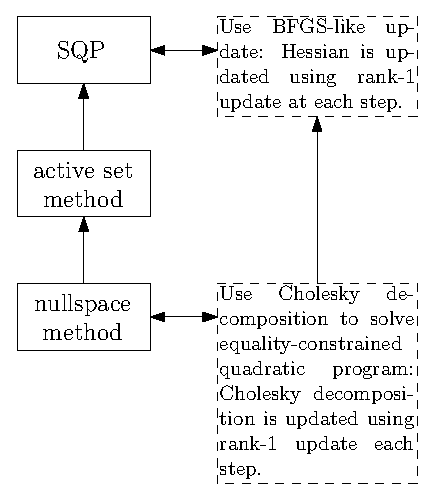
\includegraphics{constrained-newton.eps}
% \end{center}

% \paragraph{A quick thought about complexity.} It looks like it will be
% difficult to push the worse-case bound for the ``updating'' version of
% the algorithm down from $O(kd^2)$. But what is the expected number of
% active constraints? The outer update will always need $O(d^2)$ per
% iteration, but the iterations for the inner products might be
% smaller. E.g., if $\mu = E[m]$, then a matrix multiplication or
% triangular solve would require $O(\mu d)$. If
% $\mu = O(d^{1 - \epsilon})$ for $\epsilon \in (0, 1)$, say, then we
% would have made a reasonable to $O(d^{1 + \epsilon}) = o(d^2)$.

% Also, if $D$ is the dimension of the problem, if we assume that the
% number of iterations is $K(d) = O(1)$ for each subproblem of dimension
% $d \leq D$, then using the approach above combined with the
% hierarchical update would let us perform the entire update in:
% \begin{align*}
%   \sum_{d=0}^D d^2 = \frac{D(D + 1)(2D + 1)}{6} = \frac{D^3}{3} + O(D^2)
% \end{align*}
% operations.

\end{document}

%%% Local Variables:
%%% mode: latex
%%% TeX-master: t
%%% End:
